\documentclass[11pt]{article}
\usepackage{amsmath,amsthm,amsfonts,amssymb,amscd}
\usepackage{multirow,booktabs}
\usepackage[table]{xcolor}
\usepackage{fullpage}
\usepackage{lastpage}
\usepackage{enumitem}
\usepackage{fancyhdr}
\usepackage{mathrsfs}
\usepackage{wrapfig}
\usepackage{setspace}
\usepackage{calc}
\usepackage{multicol}
\usepackage{cancel}
\usepackage[retainorgcmds]{IEEEtrantools}
\usepackage[margin=3cm]{geometry}
\usepackage{amsmath}
\newlength{\tabcont}
\setlength{\parindent}{0.0in}
\setlength{\parskip}{0.05in}
\usepackage{empheq}
\usepackage{framed}
\usepackage[most]{tcolorbox}
\usepackage{xcolor}
\usepackage{listings}
\usepackage{graphicx}
\graphicspath{images/}
\definecolor{mygray}{rgb}{0.5,0.5,0.5}
\colorlet{shadecolor}{orange!15}
\parindent 0in
\parskip 12pt
\geometry{margin=1in, headsep=0.25in}
\theoremstyle{definition}
\newtheorem{defn}{Definition}
\newtheorem{reg}{Rule}
\newtheorem{exer}{Exercise}
\newtheorem{note}{Note}
\begin{document}
\setcounter{section}{0}
\title{CS 491/691 Project 1}

\thispagestyle{empty}

\begin{center}
{\LARGE \bf CS 491/691 Project 2}\\
{\large Elaine Chu and Jared Manning}\\
Fall 2019
\end{center}

\textbf{Note: The following functions are implemented with the \textsf{numpy}, \textsf{random}, and \textsf{statistics} functions}.

\section{Nearest Neighbors}
\subsection{KNN\_test}
Takes in training data sample features \textsf{X\_train}, training data sample labels \textsf{Y\_train}, test data sample features \textsf{X\_test}, test data labels \textsf{Y\_test}, and number of neighbors to test on, \textsf{K} and returns the accuracy of the classifier on the test data.

\begin{enumerate}
 \item Initial steps
 \begin{enumerate}
    \item First, we add a fail-safe to return the accuracy as 0 if K is defined as 0. We also stored the \textsf{total} number of samples and started the \textsf{counter} as 0.
\begin{lstlisting}[language=python, frame=single]
def KNN_test(X_train, Y_train, X_test, Y_test, K):
    if K == 0:
    	return 0
    total = len(X_test)
    correct = 0
\end{lstlisting}    
    \end{enumerate}
 \item Loop through all the samples in test data
 \begin{enumerate}
     \item The next step is starts the bulk of the function, and begins with a \textsf{for loop} that iterates through all of the test data. For each test sample, empty lists are initiated to be filled later on in the analysis. The maximum distance of the test data from a nearest neighbor, \textsf{max\_dist}, is set to 0, and the index of the furthest nearest neighbor, \textsf{max\_idx}, is set to NULL. 
\begin{lstlisting}[language=python, frame=single]
for sample_idx, sample in enumerate(X_test):
    dists = []
    dist_idxs = []
    max_dist = 0
    max_idx = None
\end{lstlisting}

 \item Loop through all the samples in training data and find the neighbor (\textsf{K}) closest to the test sample
 \begin{enumerate}
     \item At this step, iterate through all of the samples in training data, setting the distance, \textsf{dist}, to 0.
\begin{lstlisting}[language=python, frame=single]
for idx, trainData in enumerate(X_train):
	dist = 0
\end{lstlisting}
     \item Next, calculate the Euclidean distance between each training feature to test feature. The square root is left out of the calculation, because it is not necessary for comparing distances in this instance. 
\begin{lstlisting}[language=python, frame=single]
for feat_idx in range(0,len(trainData)):
    dist += (sample[feat_idx] - trainData[feat_idx]) 
        * (sample[feat_idx] - trainData[feat_idx])
\end{lstlisting}
     \begin{enumerate}
     \item Calculated distance is then stored as \textsf{dist} for the \textsf{feat\_idx}-th sample in the training data.
     \end{enumerate}
    \item If the list of distances, \textsf{dists}, is less than the defined \textsf{K}, for number of nearest neighbors, add the distance of the current training sample, \textsf{dist}, to \textsf{dists}, and add the current traning sample's index, \textsf{idx}, to the list of distance indices, \textsf{dist\_idx}.
\begin{lstlisting}[language=python, frame=single]
if len(dists) < K:
    dists += [dist]
    dist_idxs += [idx]
    if dist > max_dist:
    	max_dist = dist
    	max_idx = idx
\end{lstlisting}
    \begin{enumerate}
        \item If the distance between the current training and test sample is greater than value of \textsf{max\_dist}, code \textsf{max\_dist} as \textsf{dist}, and recode \textsf{max\_idx} as \textsf{idx}. This defines the current distance between the training sample and test sample as the greatest distance between any training sample and the current text sample.
    \end{enumerate}
    \item If \textsf{dist} is less than \textsf{max\_dist}, then replace \textsf{max\_dist} from the list of distances and list of distance indices for the current test sample with \textsf{dist}. Reset \textsf{max\_dist} as the largest value in the list \textsf{dists} and the corresponding index in \textsf{dist\_idxs}.
\begin{lstlisting}[language=python, frame=single]
elif dist < max_dist:
    dists.remove(max_dist)
    dist_idxs.remove(max_idx)
    dists += [dist]
    dist_idxs += [idx]
    max_dist = max(dists)
    max_idx = dist_idxs[dists.index(max_dist)]
    \end{lstlisting}
 \end{enumerate}
\end{enumerate}
\item Iterate through the K nearest neighbors and calculate the majority vote
 \begin{enumerate}
     \item First, define the number of positive and negative votes as 0. Define the \textsf{decision} as NULL.
\begin{lstlisting}[language = python, frame = single]
pos_votes = 0
neg_votes = 0
decision = None
\end{lstlisting}
    \item Next, iterate through the K nearest neighbors and calculate the majority vote to determine whether the \textsf{decision} is positive or negative.
\begin{lstlisting}[language=python, frame=single]
for i in dist_idxs:
    if Y_train[i][0] == 1:
    	pos_votes+=1
    else:
    	neg_votes+=1
    if pos_votes > neg_votes:
    decision = 1
    else:
    decision = -1
\end{lstlisting}
        \begin{enumerate}
            \item If the number of positive votes is greater than the number of negative votes, then \textsf{decision} is positive, whereas the opposite returns \textsf{decision} as negative.
        \end{enumerate}
        \item If the \textsf{decision} matches the test label from \textsf{Y\_test}, then add 1 to the \textsf{correct} counter.
\begin{lstlisting}[language=python, frame=single]
if decision == Y_test[sample_idx][0]:
	correct+=1
\end{lstlisting}
\end{enumerate}
\item Calculate the accuracy of \textsf{K} nearest neighbors
    \begin{enumerate}
        \item Divide the number of\textsf{correct} classifications by the \textsf{total} number of test samples. Return the accuracy.
    \end{enumerate}
\begin{lstlisting}[language=python, frame=single]
return correct/total
\end{lstlisting}
\end{enumerate}

\subsection{Write-Up}
\begin{shaded}
Using the following training data, how would your algorithm classify the test points listed below
with \textsf{K=1}, \textsf{K=3}, and \textsf{K=5}?
\begin{center}
    \begin{tabular}{|c|c|c|c|c|c|}
    \hline
    \rowcolor{gray!15}X1 & X2 & Label & K=1 & K=3 & K=5\\
    \hline
    \rowcolor{white}1   &   1   &   1   &   -1  &   -1  &   1\\
    \rowcolor{white}2   &   1   &   -1  &   1   &   1   &   -1\\
    \rowcolor{white}0   &   10  &   1   &   1   &   1   &   -1\\
    \rowcolor{white}10  &   10  &   -1  &   -1  &   1   &   -1\\
    \rowcolor{white}5   &   5   &   1   &   -1  &   -1  &   -1\\
    \rowcolor{white}3   &   10  &   -1  &   1   &   -1  &   -1\\
    \rowcolor{white}9   &   4   &   1   &   1   &   1   &   1\\
    \rowcolor{white}6   &   2   &   -1  &   1   &   1   &   1\\
    \rowcolor{white}2   &   2   &   1   &   -1  &   -1  &   1\\
    \rowcolor{white}8   &   7   &   -1  &   1   &   1   &   1\\
    \hline
    \end{tabular}  
\end{center}
\end{shaded}

\subsection{choose\_K}
This function takes in training and validation data, and returns the number of \textsf{K} nearest neighbors that produces the highest classification accuracy for the validation data.
\begin{enumerate}
    \item Initial steps
    \begin{enumerate}
        \item Set values \textsf{best\_acc} and \textsf{best\_K} as 0.
\begin{lstlisting}[language=python, frame=single]
best_acc = 0
best_K = 0
\end{lstlisting}
    \end{enumerate}
    \item Loop through all possible values of \textsf{K}
    \begin{enumerate}
        \item This block of code loops through all odd values of \textsf{K} and runs the previously implemented \textsf{KNN\_test} with training and validation data as inputs, storing the accuracy as \textsf{acc}. Next, evaluate if accuracy is greater than \textsf{best\_acc}. If TRUE, replace best accuracy with the current accuracy, and replace \textsf{best\_K} with the current \textsf{K} value. Once finished looping, return \textsf{best\_K}.
\begin{lstlisting}[language=python, frame=single]
for i in range(1,len(X_train)+1):
    #if its even skip (K should be odd)
    if i%2 == 0:
    	continue
    acc = KNN_test(X_train, Y_train, X_val, Y_val, i)
    if acc > best_acc:
    	best_acc = acc
    	best_K = i
return best_K
\end{lstlisting}
        \begin{enumerate}
            \item All possible values of \textsf{K} range from 1 to the number of samples there are in the training data. \textsf{K=1} results in overfitting and \textsf{K=N} results in underfitting, which are the most extreme cases.
            \item Skip even values of \textsf{K} to avoid the possibility of a tie.
        \end{enumerate}
    \end{enumerate}
\end{enumerate}

\subsection{Write-Up}
\begin{shaded}
What is the best K value for the training data above?
Answer: K=9, Accuracy = 0.7
\end{shaded}

\clearpage
\section{Clustering}
\subsection{K\_Means}
This function takes feature vectors \textsf{X} and a \textsf{K} value as input and returns a numpy array of cluster centers C. 
\begin{enumerate}
    \item Initial steps
        \begin{enumerate}
            \item This initial step stores the number of samples (\textsf{num\_samps}) as the number of rows in \textsf{X}. It also initializes random cluster centers by randomly choosing \textsf{K} index numbers of samples from \textsf{X}.
\begin{lstlisting}[language=python, frame=single]
num_samps = X.shape[0]

cluster_index = random.sample(range(num_samps),K)
newlabels = []
clusters = []
old_clusters = [0] * K

for a in range(K):
    clusters.append(list(X[cluster_index[a]]))
\end{lstlisting}
    \begin{enumerate}
        \item This step also initializes \textsf{newlabels} and \textsf{clusters} as empty lists, and \textsf{old\_clusters} as a list \textsf{K} elements long, filled with 0.
        \item After the empty \textsf{clusters} list is initialized, a for loop fills it with the randomly selected cluster centers.
    \end{enumerate}
    \end{enumerate}
    \item Update cluster centers
    \begin{enumerate}
        \item This next block represents the bulk of the \textsf{K\_Means} code within a for loop. First, update cluster centers \textbf{many} times, until the they stop changing between loops.
\begin{lstlisting}[language=python, frame=single]
for i in range(999): 
    if old_clusters == clusters:
        break
\end{lstlisting}
        \item If clusters change between loops, recode \textsf{old\_cluster} as the last cluster centers and reinitialize \textsf{clusters} as an empty list. Begin a loop that iterates through all samples in \textsf{X}. 
\begin{lstlisting}[language=python, frame=single]
for b in range(num_samps):  # loop through samples
    samp = X[b]  # select sample
    centroid_dist = []
\end{lstlisting}
            \begin{enumerate}
                \item Here, initiate \textsf{samp} as the current sample. Also initiate an empty list, \textsf{centroid\_dist}.
            \end{enumerate}
        \item Next, loop through \textsf{centroids} to calculate Euclidean distances (except for square-root) from cluster centers to \textsf{samp}. Store the distances in \textsf{centroid\_dist}.
\begin{lstlisting}[language=python, frame=single]
for c in range(K):  # loop through centroids
    centroid = old_clusters[c]
    samp_dist = np.square(samp - centroid)
    summed_dist = np.sum(samp_dist)
    centroid_dist.append(summed_dist)

best_clust = centroid_dist.index(min(centroid_dist))
newlabels.append(best_clust)
\end{lstlisting}
        \begin{enumerate}
            \item Outside of the loop, find the smallest distance, and declare that cluster center as the closest to \textsf{samp}. Store the cluster center index as the cluster label for the current sample. 
        \end{enumerate}
    \end{enumerate}
    \item Calculate new cluster centers
    \begin{enumerate}
        \item This next step takes the \textsf{newlabels} of each sample in \textsf{X} and calculates new cluster centers given the samples closest to each old cluster center.
\begin{lstlisting}[language=python, frame=single]
for d in range(K):
    index_list = np.where(np.asarray(newlabels)==d)[0]
        clusters.append(old_clusters[d])
    if len(index_list) == 0:
        clusters.append(old_clusters[d])
        clusters = sorted(clusters)
    else:   
        new_mean = np.nanmean(X[index_list,], axis=0)
        clusters.append(tuple(new_mean))
        clusters = sorted(clusters)
newlabels = []
\end{lstlisting}
        \begin{enumerate}
            \item The \textbf{if statement} considers whether any of the new cluster centers have returned as 'nan'. If so, old clusters centers replace the 'nan' to prevent warnings.
            \item New cluster centers are calculated as the mean of the samples closest to the old cluster centers. The list of cluster centers, \textsf{clusters}, is sorted to allow for uniform comparison between loops.
            \item Outside of the for loop, \textsf{newlabels} is reinitialized as an empty list.
        \end{enumerate}
    \end{enumerate}
    \item Return best cluster centers
    \begin{enumerate}
        \item This step outside of all for loops returns the best cluster centers, only computing after cluster centers stop changing within the overarching for loop from \textbf{Step 2}.
\begin{lstlisting}[language=python, frame=single]
C = clusters
C = np.array(C)
return C
\end{lstlisting}
        \begin{enumerate}
            \item This step also converts the output into an \textsf{numpy} array, as asked.
        \end{enumerate}
    \end{enumerate}
\end{enumerate}

\clearpage
\subsection{Write-Up}
\begin{shaded}
Test your function on the following training data, with K=2 and K=3. Plot the clusters in different colors and label the cluster centers.
\end{shaded}

\begin{figure}[hbt!]
 \centering
 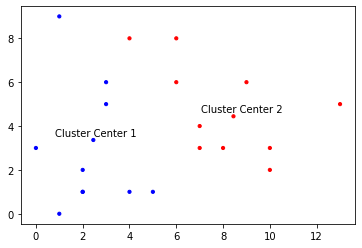
\includegraphics[scale=0.90]{Clustering_plot1}
\end{figure}
\textbf{Figure 1.} The above figure represents the classifications of training data using \textsf{K\_Means}, given K=2. 

\begin{figure}[hbt!]
 \centering
 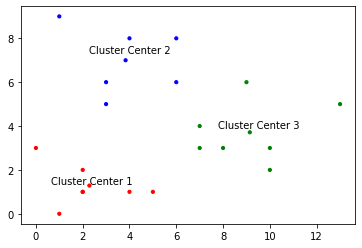
\includegraphics[scale=0.90]{Clustering_plot2}
\end{figure}
\textbf{Figure 2.} The above figure represents the classifications of training data using \textsf{K\_Means}, given K=3. 
\\
\\
\textbf{Note:} These plots are representative of just one of the outputs given by \textsf{K\_Means}. Because the initial clusters vary each time, resulting cluster centers can vary.

\subsection{K\_Means\_better}
This function takes feature vectors \textsf{X} and a \textsf{K} value as input and returns a numpy array of cluster centers, \textsf{C}.
\begin{enumerate}
    \item Initial Steps
    \begin{enumerate}
        \item First, initiate an empty list of clusters, \textsf{cluster\_list}
\begin{lstlisting}[language=python, frame=single]
cluster_list = []
\end{lstlisting}
    \end{enumerate}
    \item Calculate cluster centers
    \begin{enumerate}
        \item Here, calculate cluster centers \textbf{many} times, append cluster centers to \textsf{cluster\_list}.
\begin{lstlisting}[language=python, frame=single]
for i in range(1000):
    C = K_Means(X,K)
    C = [tuple(s) for s in C]
    cluster_list.append(C)
\end{lstlisting}
    \end{enumerate}
    \item Return the majority rules cluster
    \begin{enumerate}
        \item Here, convert individual entries of \textsf{cluster\_list} to tuples to allow for comparison of cluster centers. Find the most common cluster center, and store as \textsf{mode\_cluster}. Convert \textsf{mode\_cluster} to a numpy array as required. Return \textsf{mode\_cluster}.
\begin{lstlisting}[language=python, frame=single]
final_list = [tuple(t) for t in cluster_list]

mode_cluster = stat.mode(final_list)
mode_cluster = np.array(mode_cluster)

return mode_cluster
\end{lstlisting}
    \end{enumerate}
\end{enumerate}

\clearpage
\subsection{Write-Up}
\begin{shaded}
Test your function on the following training data, with K=2 and K=3. Plot the clusters in different colors and label the cluster centers.
\end{shaded}

\begin{figure}[hbt!]
 \centering
 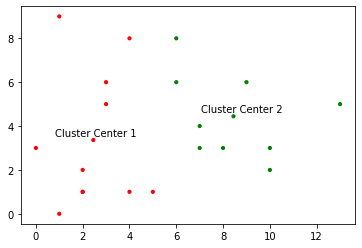
\includegraphics[scale=0.90]{Clustering_plot3}
\end{figure}
\textbf{Figure 3.} The above figure represents the classifications of training data using \textsf{K\_Means\_better}, given K=2. 

\begin{figure}[hbt!]
 \centering
 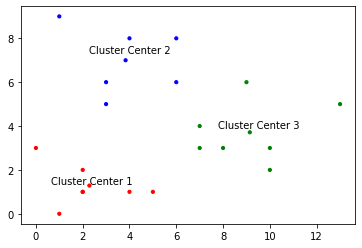
\includegraphics[scale=0.90]{Clustering_plot4}
\end{figure}
\textbf{Figure 4.} The above figure represents the classifications of training data using \textsf{K\_Means\_better}, given K=3. 

\section{Perceptron}
\subsection{perceptron\_train}
This function takes training data features \textsf{X} and labels \textsf{Y}, and returns \textsf{[w,b]}, a list containing a list of weights, \textsf{w} and the bias, \textsf{b}.
\begin{enumerate}
    \item Initial steps
    \begin{enumerate}
        \item First, initialize weights, \textsf{w}, as a vector of zeros and bias, \textsf{b}, as 0. Set variable \textsf{updated} as TRUE.
\begin{lstlisting}[language=python, frame=single]
w = [0] * len(X[0])
b = 0
updated = True
\end{lstlisting}
\end{enumerate}
\begin{enumerate}
    \item Update weights, \textsf{w}, and bias, \textsf{b}
    \begin{enumerate}
        \item Next, run a for loop until all samples are correctly classified without updating.
    \end{enumerate}
\begin{lstlisting}[language=python, frame=single]
while updated:
    updated = False
    
    for sample_idx, x in enumerate(X):
    	a = b
    	for feat_idx, feat in enumerate(x):
    		a += w[feat_idx] * feat
    
    	if a * Y[sample_idx][0] <= 0:
    		updated = True
    		for feat_idx, feat in enumerate(x):
    			w[feat_idx] += feat * Y[sample_idx][0]
    		b += Y[sample_idx][0]
    return [w,b]
\end{lstlisting}
        \begin{enumerate}
            \item To do so, the code continues to run as long as \textsf{updated = TRUE}.
            \item Variable \textsf{a} is calculated for each sample. If \textsf{a} and label \textsf{Y} are not the same, then weights and bias is updated.
        \end{enumerate}
    \end{enumerate}
\end{enumerate}

\clearpage
\subsection{perceptron\_test}
This function takes test data features \textsf{X\_test} and labels \textsf{Y\_test}, weight vector \textsf{w}, and bias, \textsf{b}, and returns the accuracy of the perceptron on the test data.
\begin{enumerate}
    \item Initial steps
    \begin{enumerate}
        \item First, set \textsf{total} as the number of samples in \textsf{X\_test}, and set the counter, \textsf{correct}, as 0.
    \end{enumerate}
\begin{lstlisting}[language=python, frame=single]
total = len(X_test)
correct = 0
\end{lstlisting}
    \item Calculate \textsf{a} for each sample
    \begin{enumerate}
        \item Next, this bulk of code calculates \textsf{a} for each sample using the inputted weights, \textsf{w}, and bias, \textsf{b}. If \textsf{a} is greater than 1, the sample \textsf{decision} as a 1, otherwise as a -1.
\begin{lstlisting}[language=python, frame=single]
for idx, x in enumerate(X_test):
    decision = None
    a = b
    for feat_idx,feat in enumerate(x):
    	a += w[feat_idx] * feat

    if a > 0:
    	decision = 1
    else:
    	decision = -1
\end{lstlisting}
    \end{enumerate}
\begin{enumerate}
    \item Calculate accuracy of perceptron
    \begin{enumerate}
        \item If the perceptron classification, \textsf{decision}, is the same as the sample label, \textsf{Y\_test}, then add 1 to the \textsf{correct} counter. Return the accuracy at the end, which is \textsf{correct / total}.
    \end{enumerate}
\begin{lstlisting}[language=python, frame=single]
	if decision == Y_test[idx][0]:
		correct+=1
return correct/total
\end{lstlisting}
\end{enumerate}
\end{enumerate}

\clearpage
\subsection{Write-Up}
\begin{shaded}
Train your perceptron on the following dataset. Using the w and b you get, plot the decision boundary.

\begin{center}
\textsf{w = [2.0, 4.0]} and \textsf{b = 2}
\\
\textsf{decision boundary = -0.5x – 0.5}  
\\
Accuracy = 1.0
\end{center}
\end{shaded}

\begin{figure}[hbt!]
 \centering
 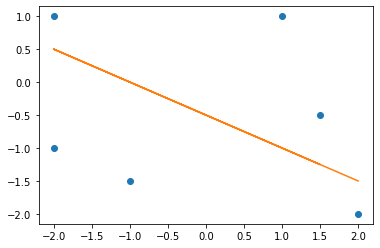
\includegraphics[scale=0.90]{Perceptron_plot}
\end{figure}
\textbf{Figure 5.} The above figure represents the decision boundary using \textsf{w} and \textsf{b} from \textsf{perceptron\_train}.
 
\end{document}